\section{Background on Rational Proofs}
\begin{frame}{Overview of Rational Proofs [AM12]}
\begin{itemize}[<+- | alert@+>]
	\item A variant of interactive proofs where the verifier pays the prover at the end;
	\item \textbf{Soundness:}
	\begin{itemize}
		\item ``A cheating worker gains less than an honest one''
	\end{itemize}
%	\item Other desiderata:
%	\begin{itemize}
%		\item Reward should be higher than cost (\textit{individually rational})
%		\item Ensuring ``significant'' losses for cheaters;
%		\item Ensuring ``compact'' budget for delegators.
%	\end{itemize}
\end{itemize}
\onslide<1->
\begin{figure}
	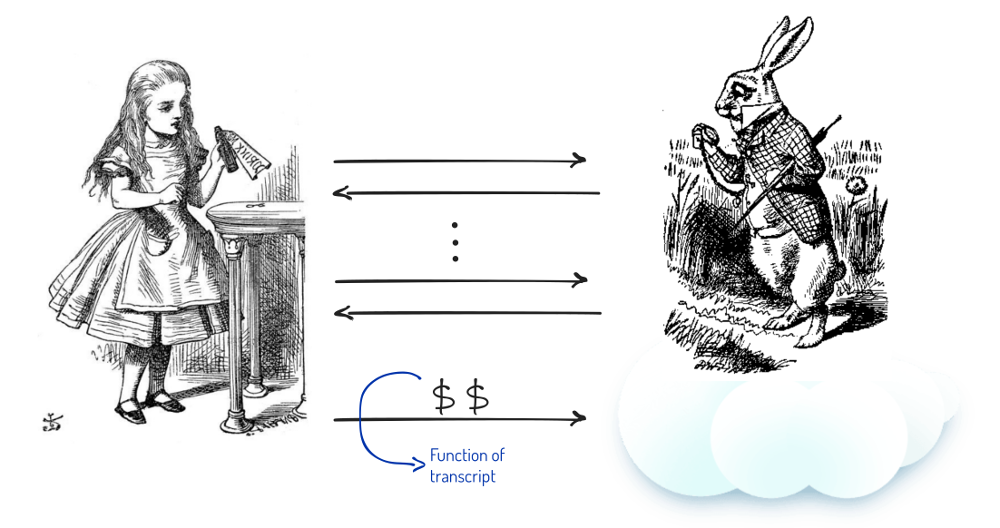
\includegraphics[scale=0.23]{pics/interaction.png}
\end{figure}
% Recall interactive proofs
% Recall our goal
\end{frame}


\begin{frame}{Rational Proofs: Definition [AM12]}
		\begin{framed}
			Let $f$ be a function and $(P,V)$ be a pair of algorithms. $(P,V)$ is a rational proof for $f$ if both:
			\onslide<+->
			\begin{enumerate}[<+- | alert@+>]
				\item \emph{("The honest prover always replies correctly")} 
				$$ \forall x\  \Pr[output(P,V)(x) = f(x) ] = 1$$
				\item \emph{("Any other prover will earn less than the honest one")}
				$$ \forall \disP \ \forall x \  \expRewProtHon - \expRewProtDis \geq \delta_{\disP}(x)  $$
				for some reward function $\rew$ and gap $\delta_{\disP}(x) \geq 0$
			\end{enumerate}
		\end{framed}
		
		%\pause
		%\vspace{0.5cm}
		%\center{\large{\textbf{What does $\rew$ look like?}}}
\end{frame}

\section{Rational Proofs for Feasible Computation}

\begin{frame}{Rational Proofs for Space-Bounded Computations}
\begin{block}{Theorem (informal)}
	If $L$ can be decided in time $T$ and space $S$ by a $DTM$, then it admits a rational proof with $O(\log n)$ rounds, $S \log n$ communication complexity and Verifier's running time.
\end{block}
\pause
\begin{itemize}[<+->]
	\item \textit{Special case:} If $T=poly(n)$ and $S=polylog(n)$ then we have a $O(\log n)$ round protocol with a polylog verifier.
	\item Generalization to randomized computation (using PRGs against space-bounded adversaries \cite{nisan1992pseudorandom}).
	\begin{itemize}
		\item unconditional PRGs
		\item Possible through one of our composition result.
	\end{itemize}
\end{itemize}
	% TODO: Say about generalization of result
\end{frame}

\begin{frame}{RPs for Space-Bounded Computations (intuition)}
\begin{itemize}
	\item Core: interactive proof with ``low'' soundness;\pause
	\item In the end, if prover accepts, reward $R$ otherwise reward $0$
\end{itemize}
\medskip
\begin{figure}
	
\includegraphics[scale=0.3]{pics/space-protocol.png}
	\caption{Configuration Graph of a deterministic computation}
\end{figure}
\end{frame}

\begin{frame}{How Efficient Can We Hope RPs for P to be?}
	\textbf{Our result for space-bounded (prev. slides):} For $S = \polylog(n)$ we have a polylog verifier and polylog total communication.
	\pause
	\begin{block}{Theorem (informal)}
It is unlikely\footnote{Unless ``something related'' to $\NP \subseteq \BPP$ holds} there exist rational proofs for P with polylog verification and log total communication;
\end{block}
\end{frame}

